%!TEX root = ../Thesis.tex

\section{Epoch Alignment}

A single sample of pseudoranges from any two receivers will not be taken at the exact same time without a connecting network to implement control. This increases the setup requirements which in turn increases the cost of the system and reduces the ease of compatibility with different receivers. The earliest time between all the receivers will be used as the time reference point called common epoch. The satellite position in the future time steps were backcalculated to find the difference in the pseudorange. The time between receivers would be a maximum of one second, as the slowest sampling time is typically 1 Hz. This extra distance is only in the vacuum of space and is not affected by potential nonlinear affects such as ionosphere and troposphere errors that affect the speed of light.\\

\subsection{Satellite Time}
The known variables from the raw GPS data is the time the sample measurement was taken $t_\omega$ and the pseudorange to each visible satellite $\rho_\omega^1$ for each receiver $\omega$.


The error in the normal vector due to the time difference is

By the distributive law
\begin{eqnarray}
\hat{\eta}\cdot s + \hat{\eta}\cdot v = |\eta| 
\end{eqnarray}
\begin{eqnarray}
\Delta \rho &=& |\eta| - |v|\\ % check -ves
&=& \hat{\eta}\cdot s + \hat{\eta}\cdot v - |v|\\
&=& \hat{\eta}\cdot s + |\hat{\eta}||v|\cos(\theta) - |v| \label{Eq:deltarho}
\end{eqnarray}
As |v| is >20 000 km and s is <4 km, $\theta\approx 0$ which means $\cos\theta\approx1$. The magnitude of a unit vector is one therefore \eqref{Eq:deltarho} simplifies to
\begin{eqnarray}
\Delta\rho = \hat{\eta}\cdot s 
\end{eqnarray}


The vector $s$ is the transform of the satellite from time $t_2$ to the common epoch time $t_1$. It is calculated using the 

$t_1 = distance/c for alpha receiver$ 
$t_2 = t_{sampleoffset}- |v|/c$

The vector $v$ is the measured pseudorange of a receiver from a particular visible satellite at $t_2$ with an unknown direction vector. The direction vector is unknown because the position of the receiver is what is being solved for. The vector $\eta$ describes the known direction vector from the single approximate location of the geographic region to the common epoch of a particular visible satellite. It is the magnitude of $\eta$ that describes what the pseudorange would have been if the measurement was taken at the common epoch. The difference between the  $|\eta|-|v|$

Because of the asynchronous time, some of the satellite correlated errors would not correlate as well as if it was from the same point in time. This is because the path through the ionosphere and troposphere is not exactly the same. 

%Error as the clock bias is unknown at this point. In the literature, an approximate clock bias is calculated through NLLS first then the epoch is transformed to process an updated pseudorange. The updated pseudorange is then used again in NLLS and the process is repeated until convergence is reached.

\begin{figure}
\centering
\caption{Vector Epoch Synchronisation}
\label{Fig:epochsync}
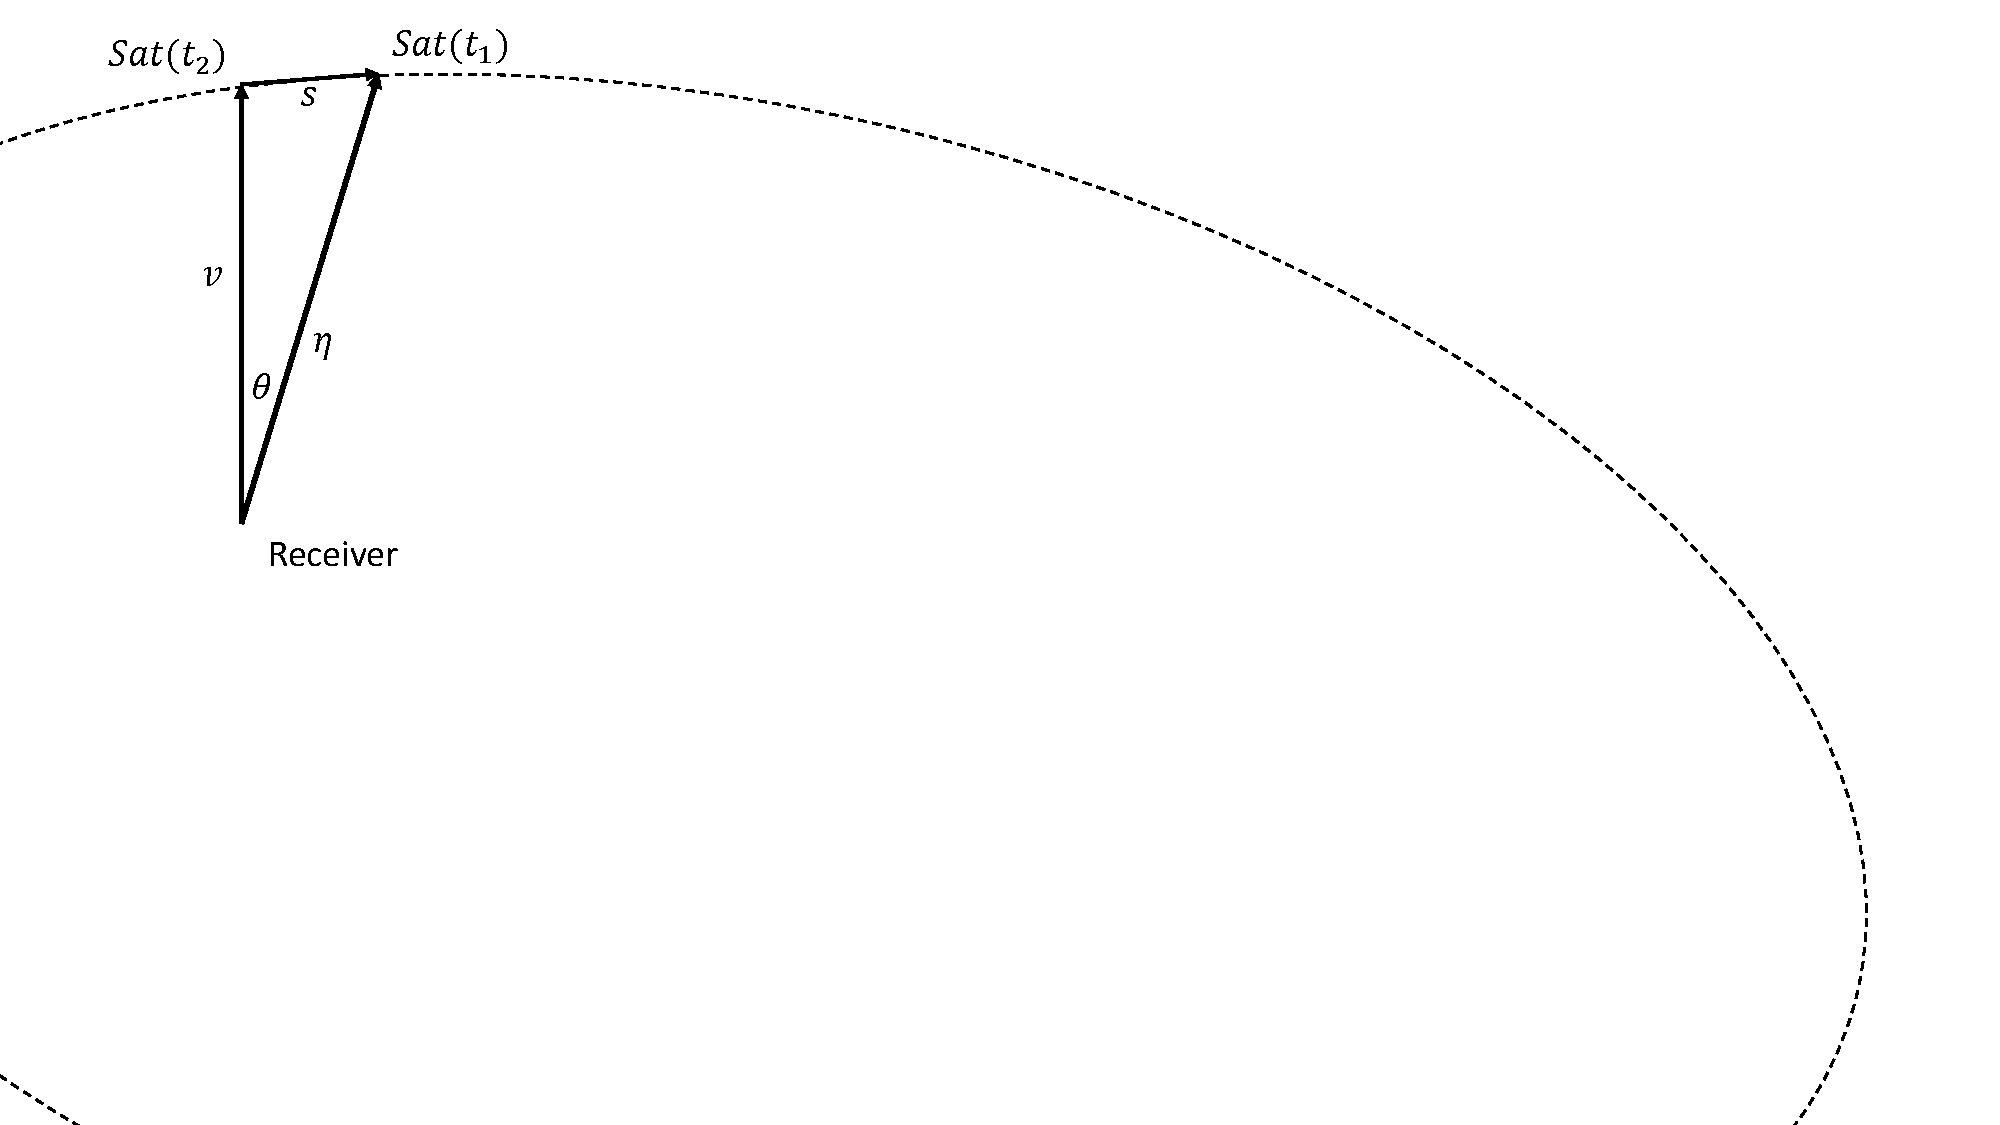
\includegraphics[trim=0 10cm 23cm 0,clip,width=0.6\linewidth]{ChapterPerception/Figures/epochalignment.pdf}
\end{figure}

% type up maths for this assumption- thats it - not an assuption, this goes into the algorithm- assumption is the asynch time described by (sample offset-time of flight) has error in position of satellite as there is error in time of flight - or do you know position of sat when sent????????








